\documentclass{article}
\usepackage[spanish]{babel}
\usepackage{amsmath}
\usepackage{physics}
\usepackage{graphicx}
\usepackage{subfigure}
\graphicspath{{/home/vian/0_uam/1_TFG/latex/img/}}

\title{Desarrollo}

\begin{document}

\maketitle{}

\section{Primer grafo}  % TODO: Cambiar nombre
\label{sec:4-primer grafo}

\begin{figure}[htbp]
  \centering
  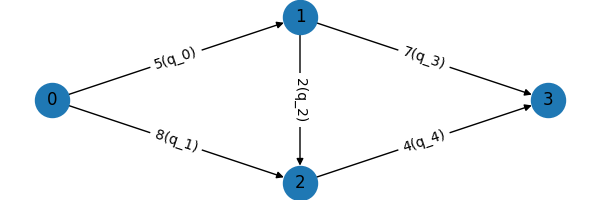
\includegraphics[scale=0.75]{primer_grafo/primer_grafo}
\end{figure}

Con este grafo se pretenden analizar los resultados obtenidos en la sección 2.2 (\textit{Single-Objective Quantum Routing Optimization}) del artículo \cite{multi-objective_routing_optimization}.

El problema a resolver es encontrar el camino más corto que conecte los nodos \textit{0} y \textit{3}.
\begin{itemize}
\item \textbf{Objetivo:}
  \begin{align*}
    &min(5X_{01} + 8X_{02} + 2X_{12} + 7X_{13} + 4X_{23}) \\
    &\textnormal{dde } X_{ij} = \begin{cases}
      1 \textnormal{ si el camino contiene a la arista del nodo \textit{i} al \textit{j}} \\
      0 \textnormal{ en otro caso}
    \end{cases}
  \end{align*}
  
\item \textbf{Restricciones:}
  También se deben añadir una serie de restricciones para evitar caminos triviales o incongruentes.

  \begin{equation}
    X_{01} + X_{02} = 1
  \end{equation}
  \begin{equation}
    \begin{split}
      X_{01} = X_{12} + X_{13} \\
      X_{02} + X_{12} = X_{23}
    \end{split}
  \end{equation}

  Estas restricciones se pueden justificar como:
  \begin{enumerate}
  \item Debe haber exactamente un eje del camino que involucre al nodo de comienzo. Obliga al camino a comenzar por dicho nodo.
  \item Para cada nodo intermedio debe haber en el resultado tantas aristas entrantes como salientes. Evita caminos incongruentes y hace que el único nodo posible para finalizar sea el nodo final.
    
  \end{enumerate}
  Siguiendo el caso del artículo se elige como valor del \textit{modificador de Lagrange} \(P=27\), ya que debe ser estrictamente mayor que el máximo de la función objetivo:
  \(\max_{x}{f_{\textnormal{sin restricc}}(x)} = \sum_{(i, j)\in{E}}{w_{ij}} = 26\)

\end{itemize}

De acuerdo con los pasos descritos en la sección \ref{sec:3-problemas de optimizacion combinatoria},  % TODO: citar
la función de coste clásica en su versión QUBO es:
\begin{align*}
  f(X) = &5X_{01} + 8X_{02} + 2X_{12} + 7X_{13} + 4X_{23} + &&\\
         &P(X_{01} + X_{02} - 1)^2 + P(X_{01} - X_{12} - X_{13})^2 + P(X_{02} + X_{12} - X_{23})^2
\end{align*}

El número de qubits del sistema cuántico es igual a la cantidad de variables de la función clásica, esto es, la cantidad de ejees del grafo. \\
La correspondencia entre las variables de la función clásica y el circuito es la siguiente:

\begin{center}
  \begin{tabular}{|c|c|c|c|c|}
    \hline
    X\textsubscript{01} & X\textsubscript{02} & X\textsubscript{12} & X\textsubscript{13} & X\textsubscript{23}\\
    \hline
    z\textsubscript{0} & z\textsubscript{1} & z\textsubscript{2} & z\textsubscript{3} & z\textsubscript{4}\\
    \hline
  \end{tabular}
\end{center}

De acuerdo con la sección \ref{sec:3-operador c}  % TODO: Citar
la versión Ising de la función de coste queda como:
\begin{align*}
  g(z) = &5\frac{1-z_0}{2} + 8\frac{1-z_1}{2} + 2\frac{1-z_2}{2} + 7\frac{1-z_3}{2} + 4\frac{1-z_4}{2} + &&\\
         &P(\frac{1-z_0}{2} + \frac{1-z_1}{2} - 1)^2 + P(\frac{1-z_0}{2} - \frac{1-z_2}{2} - \frac{1-z_3}{2})^2 + \\
         &P(\frac{1-z_1}{2} + \frac{1-z_2}{2} - \frac{1-z_4}{2})^2 = \\
  = & 11z_0 - 17.5z_1 - 28z_2 - 17z_3 + 11.5z_4 + \\
         &13.5(z_0z_1 - z_0z_2 - z_0z_3 + z_1z_2 - z_1z_4 + z_2z_3 - z_2z_4) + \\
         &80.5 \\
\end{align*}
\par
Con respecto al operador C: \\
\begin{itemize}
\item La igualdad se cumple para variables con valores \(\{-1, 1\}\), ya que \(z_i^2 = 1\). \\
\item Debido al postulado de medición en mecánica cuántica \cite{Nielsen_Chuang_2010} la fase global es despreciable, por lo que
  \(e^{i \gamma 80.5} \cdot e^{i \gamma H_p} = e^{i \gamma H_p}\).
\item \( Rz_i(\lambda) = exp(-i\frac{\lambda}{2}Z_i) \)
\item \( Rz_iz_j(\lambda) = exp(-i\frac{\lambda}{2}Z_i \otimes Z_j) \)
\end{itemize}

\par
De esta forma, el hamiltoniano del problema es el siguiente:
\begin{align*}
  U&(C, \gamma) = exp(-i \gamma C) = &&\\
   &Rz_0(11*2\gamma) \cdot Rz_1(-17.5*2\gamma) \cdot Rz_2(-28*2\gamma) \cdot Rz_3(-17*2\gamma) \cdot Rz_4(11.5*2\gamma) \cdot \\
   &Rz_0z_1(+13.5 * 2\gamma) \cdot Rz_0z_2(-13.5 * 2\gamma) \cdot Rz_0z_3(-13.5 * 2\gamma) \cdot Rz_1z_2(+13.5 * 2\gamma) \cdot \\
   &Rz_1z_4(-13.5 * 2\gamma) \cdot Rz_2z_3(+13.5 * 2\gamma) \cdot Rz_2z_4(-13.5 * 2\gamma)
\end{align*}

Con el operador \(U(B, \beta)\) y el vector inicial, definidos en la sección \ref{sec:3-circuito de qaoa},  % TODO: Citar
y el operador \(U(C, \gamma)\) obtenido se puede construir el circuito cuántico.

\begin{itemize}
\item \textbf{Circuito obtenido ($p=1$):}
  \begin{figure}[htbp]
    \centering
    \includegraphics[scale=0.27]{circuits/primer/primer_circuit_2gamma_p-1.png}
  \end{figure}

\item \textbf{Circuito del artículo ($p=1$):}
  \begin{figure}[htbp]
    \centering
    \includegraphics[scale=0.3]{circuits/paper/paper_circuit.png}
  \end{figure}
\end{itemize}

\subsection{Diferencias con el artículo}
El circuito obtenido teóricamente difiere del que se puede ver en la sección 2.2 del artículo \cite{multi-objective_routing_optimization}. \\
En la sección anterior se obtienen operadores con la forma \(Rz(n*2\gamma)\), mientras que en la imagen del circuito en el artículo aparecen como \(Rz(n)\).

Debido a esto, y como se busca replicar los resultados del artículo, se modifica el hamiltoniano para que sea igual al de la imagen.

% TODOO: explicar el porqué del *2 puede ser válido, pero el gamma no
%        C y 2*C tendrían el mismo estado fundamental, pero con distinta energía).
%        \gamma es incorrecto, demostrado con la construcción usando QAOAAnsatz.
%        *2:
%        \begin{align*}
%          \frac{g(z)}{2} = & \frac{11}{2}z_0 - \frac{17.5}{2}z_1 - \frac{28}{2}z_2 - \frac{17}{2}z_3 + \frac{11.5}{2}z_4 + \\
%                           & \frac{13.5}{2}(z_0z_1 - z_0z_2 - z_0z_3 + z_1z_2 - z_1z_4 + z_2z_3 - z_2z_4) + \\
%                           & \frac{80.5}{2} \\
%          \frac{f(X)}{2} = &2.5X_{01} + 4X_{02} + 1X_{12} + 3.5X_{13} + 2X_{23} + &&\\
%                           &\frac{P}{2}(X_{01} + X_{02} - 1)^2 + \frac{P}{2}(X_{01} - X_{12} - X_{13})^2 + \frac{P}{2}(X_{02} + X_{12} - X_{23})^2
%        \end{align*}

\newpage
\bibliographystyle{abbrv}
\bibliography{bibliografia}

\end{document}

%%% Local Variables:
%%% mode: latex
%%% TeX-master: t
%%% End:
